\documentclass[12pt]{article}
\usepackage[utf8]{inputenc}
\usepackage{mathpazo}
\usepackage{graphicx}
\usepackage[a4paper,width=150mm,top=20mm,bottom=27mm]{geometry}
\usepackage[english]{babel}
\usepackage{setspace}
\usepackage{ragged2e}
\usepackage{amsmath}
\usepackage{booktabs}
\usepackage{tabularx}
\usepackage{hyperref}
\usepackage{xcolor}
\usepackage{float}

\hypersetup{colorlinks=true,linkcolor=black,urlcolor=blue}

\title{
\begin{center}
{\Large \bfseries A Business Analytics Study of Advertisement Fatigue in Mobile Applications}\\[0.3cm]
{\normalsize \itshape Submitted By}\\[0.2cm]
Vijayaragunathan R, CB.SC.U4CSE23757\\
Rachit Anand, CB.SC.U4CSE23139\\
Abishek R, CB.EN.U4CCE23003\\
Krishnan S., CB.SC.U4CSE23628\\
A GOWSHIK, CB.SC.U4CSE23701\\[0.4cm]
{\normalsize \itshape in partial fulfilment of the requirements for the degree of}\\[0.2cm]
{\large \bfseries BACHELOR OF TECHNOLOGY}\\
{\large \bfseries IN}\\
{\large \bfseries COMPUTER SCIENCE AND ENGINEERING}\\[0.3cm]
\includegraphics[width=0.25\textwidth]{logo_square.png}\\[0.3cm]
{\normalsize \itshape Under the Guidance of}\\[0.2cm]
Vedaj J Padman\\
{\small Assistant Professor (Sl.Gd.)}\\
{\small School of Computing, Coimbatore}\\[0.4cm]
{\normalsize \bfseries DEPARTMENT OF COMPUTER SCIENCE AND ENGINEERING}\\
{\normalsize \bfseries AMRITA SCHOOL OF COMPUTING}\\
{\normalsize \bfseries AMRITA VISHWA VIDYAPEETHAM}\\
{\normalsize \bfseries COIMBATORE - 641112}
\end{center}
}
\date{}

\begin{document}

\maketitle

\begin{center}{\Large \bfseries ABSTRACT}\end{center}
\onehalfspacing\justifying

This project analyzes advertisement fatigue in mobile applications using business analytics. Primary data was collected through a Google Forms survey (422 responses) capturing user demographics, ad exposure, and behavioral reactions. Secondary data consisted of Google Play Store reviews collected via web scraping and processed through an NLP pipeline for sentiment analysis and keyword detection. An Advertisement Fatigue Index (AFI) was derived from Likert-scale responses. Machine learning regression models, K-Means clustering, and Prophet-based time-series forecasting were applied to generate insights. An interactive dashboard was built to communicate findings to stakeholders.

\newpage\tableofcontents\newpage
\listoftables\newpage
\listoffigures\newpage

% ======================================================
\section{Introduction}
% ======================================================

Mobile applications rely heavily on digital advertising as a primary revenue source. Formats such as banner ads, interstitial ads, and rewarded video ads allow developers to offer free services while generating income. However, excessive advertising leads to advertisement fatigue — a state of annoyance and disengagement that causes users to close or uninstall applications.

This project applies a full business analytics pipeline to study advertisement fatigue, combining survey analysis, NLP-based sentiment mining, machine learning prediction, user clustering, and time-series forecasting to generate actionable insights for mobile app developers and digital marketers.

% ======================================================
\section{Problem Statement}
% ======================================================

Excessive advertisements disrupt user experience and lead to frustration, reduced engagement, and application uninstallation. Developers often lack data-driven tools to determine the optimal balance between advertisement frequency and user satisfaction.

This project addresses how business analytics techniques can quantify advertisement fatigue and identify the factors that drive user frustration, providing a basis for more effective and user-friendly advertising strategies.

% ======================================================
\section{Dataset Selection and Understanding}
% ======================================================

\subsection{Primary Dataset — Survey Data}

A structured Google Forms survey collected 422 responses (target: 1000). Variables captured include age group, gender, occupation, smartphone type, daily screen time, most used app category, advertisement frequency, ad format exposure, frustration levels (Likert scale), app closure and uninstall behavior, and willingness to pay for ad-free versions.

\subsection{Secondary Dataset — Google Play Store Reviews}

Reviews were scraped using \texttt{google-play-scraper} across multiple app categories and countries and processed through the following pipeline: \textit{Web Scraping} $\rightarrow$ \textit{Text Cleaning} $\rightarrow$ \textit{Keyword Detection} $\rightarrow$ \textit{Sentiment Classification}.

The processed dataset (\texttt{reviews\_cleaned.csv}) contains the key fields shown in Table~\ref{tab:review_fields}.

\begin{table}[H]
\centering
\begin{tabularx}{\textwidth}{lX}
\toprule
\textbf{Field} & \textbf{Description} \\
\midrule
app\_name      & Name of the application \\
category       & App category (e.g., Game, Social, Entertainment) \\
country        & Country of the reviewer \\
continent      & Continent derived from country \\
rating         & Star rating (1--5) \\
clean\_text    & Preprocessed review text \\
ad\_mentioned  & Binary flag (1 = ad keyword found) \\
ad\_keyword    & Specific ad keyword matched \\
sentiment      & Positive / Neutral / Negative \\
\bottomrule
\end{tabularx}
\caption{Fields in the Processed Review Dataset}
\label{tab:review_fields}
\end{table}

\subsection{Dashboard Dataset}

Key fields from both datasets were exported as \texttt{dashboard\_dataset.csv} and\\
\texttt{dashboard\_dataset\_survey.csv} for use in the interactive dashboard.

% ======================================================
\section{Tools and Technologies}
% ======================================================

\begin{itemize}
    \item \textbf{Python} — Core language for data analysis and modeling.
    \item \textbf{Pandas / NumPy} — Data manipulation and numerical operations.
    \item \textbf{Matplotlib / Seaborn / WordCloud} — Statistical visualizations.
    \item \textbf{NLTK / TextBlob} — NLP: text cleaning, tokenization, sentiment analysis.
    \item \textbf{google-play-scraper / tqdm} — Review scraping and progress tracking.
    \item \textbf{Scikit-learn} — Label encoding, StandardScaler, Linear/Decision Tree/Random Forest regression, K-Means clustering, PCA.
    \item \textbf{Prophet} — Time-series forecasting with daily and weekly seasonality.
    \item \textbf{React + Vite + TypeScript / TailwindCSS} — Interactive dashboard frontend.
    \item \textbf{Jupyter Notebook / Git / GitHub} — Development and version control.
\end{itemize}

% ======================================================
\section{Methodology}
% ======================================================

The project follows a nine-phase pipeline:
\begin{enumerate}
    \item Data collection (web scraping + survey)
    \item Data preprocessing (NLP cleaning, imputation, deduplication)
    \item Exploratory Data Analysis (EDA)
    \item Sentiment and text mining
    \item Ad Fatigue Index computation
    \item Machine learning regression (Ad Fatigue prediction)
    \item User segmentation (K-Means clustering + PCA)
    \item Time-series forecasting (Prophet)
    \item Business Intelligence Dashboard
\end{enumerate}

% ======================================================
\section{Data Preprocessing}
% ======================================================

\subsection{Review Data (\texttt{02\_text\_cleaning.ipynb})}

Raw reviews (\texttt{playstore\_reviews\_raw.csv}) were cleaned by removing nulls, lowercasing, stripping URLs and special characters, removing English stopwords, and retaining only alphabetic tokens. Output: \texttt{reviews\_cleaned.csv}.

\subsection{Survey Data (\texttt{05\_data\_preprocessing\_survey\_dataset.ipynb})}

The raw survey (\texttt{survey\_dataset.csv}) was preprocessed by renaming columns to snake\_case, dropping the timestamp, imputing missing values with column modes, deduplicating, and converting column types.

\subsection{Ad Fatigue Index (AFI)}

The AFI is a composite score computed as the mean of four Likert-scale columns (each mapped 1–5: Strongly Disagree → Strongly Agree):

\begin{itemize}
    \item \texttt{ads\_interrupt\_usage\_score}
    \item \texttt{ads\_cause\_frustration\_score}
    \item \texttt{ads\_reduce\_enjoyment\_score}
    \item \texttt{ads\_close\_app\_score}
\end{itemize}

AFI $\in [1, 5]$, where 1 = no fatigue, 5 = extreme fatigue. It serves as the target variable for regression and clustering.

% ======================================================
\section{Sentiment Analysis and Text Mining}
% ======================================================

\subsection{Keyword Detection (\texttt{03\_text\_mining\_sentiment.ipynb})}

A curated vocabulary of ad-related terms (\textit{ads, too many ads, ads everywhere, forced ads, pop-up ads, video ads}, etc.) was used to flag each review with a binary \texttt{ad\_mentioned} field and record the matched \texttt{ad\_keyword}.

\subsection{Sentiment Classification}

TextBlob polarity scores were used to classify each review as \textbf{Positive} (polarity $> 0$), \textbf{Negative} (polarity $< 0$), or \textbf{Neutral} (polarity $= 0$).

% ======================================================
\section{Exploratory Data Analysis}
% ======================================================

\subsection{Review Data Analysis (\texttt{04\_analysis\_and\_visualization.ipynb})}

The following visualizations were produced from the processed review dataset: overall sentiment distribution; sentiment by app name and category; ad mention frequency; rating vs. ad complaints; top 10 ad keywords; word cloud; ad complaints by category; sentiment vs. ad mentions; ad complaints by continent; and average rating by category.

Key charts are shown in Figures~\ref{fig:sent_dist}--\ref{fig:complaints_continent}.

\begin{figure}[H]
    \centering
    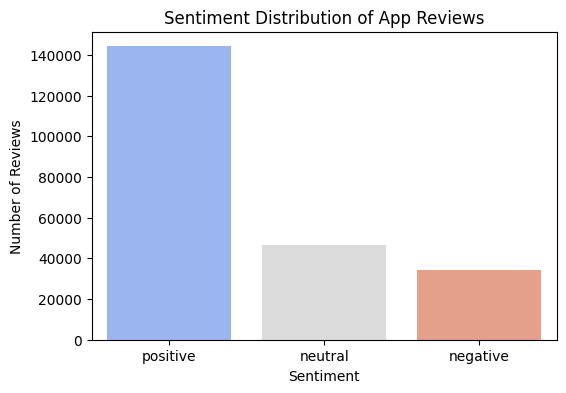
\includegraphics[width=0.85\textwidth]{reports/Sentiment Distribution of App Reviews.png}
    \caption{Sentiment Distribution of App Reviews}
    \label{fig:sent_dist}
\end{figure}

\begin{figure}[H]
    \centering
    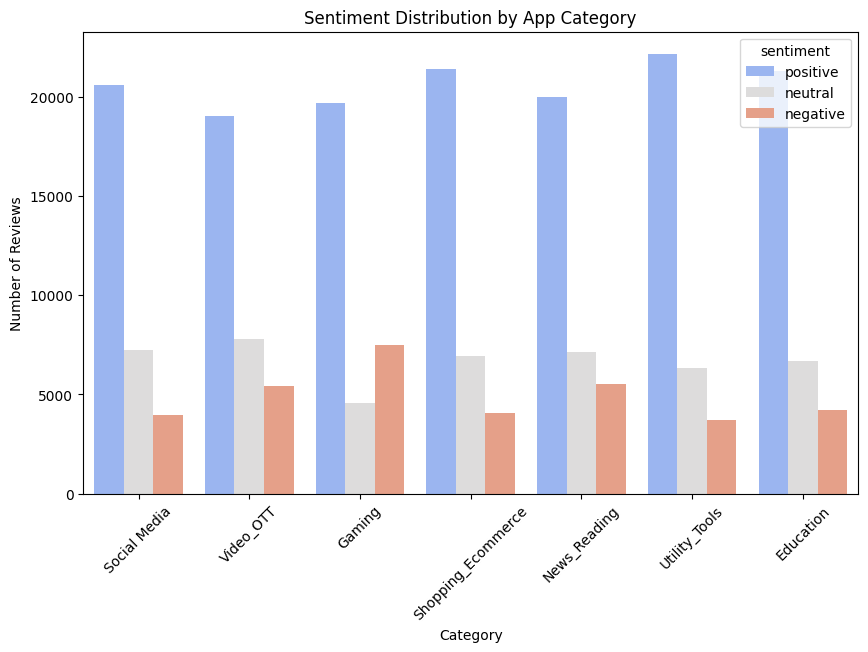
\includegraphics[width=0.85\textwidth]{reports/Sentiment Distribution by App Category.png}
    \caption{Sentiment Distribution by App Category}
    \label{fig:sent_cat}
\end{figure}

\begin{figure}[H]
    \centering
    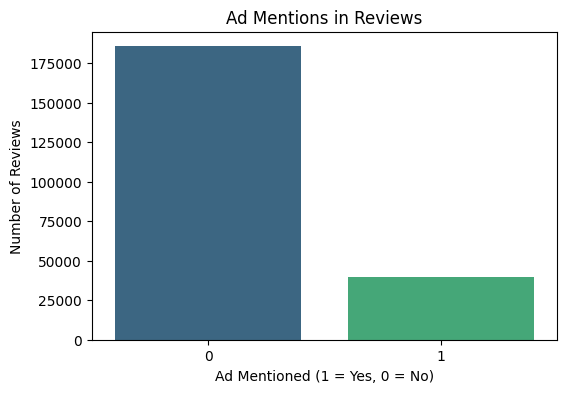
\includegraphics[width=0.85\textwidth]{reports/Ad Mentions in Reviews.png}
    \caption{Frequency of Advertisement Mentions in Reviews}
    \label{fig:ad_mentions}
\end{figure}

\begin{figure}[H]
    \centering
    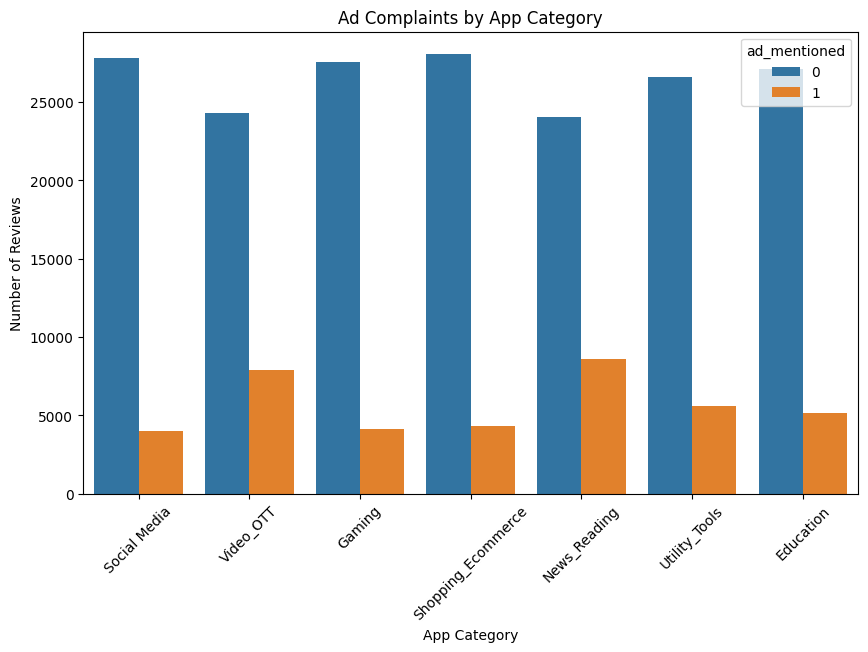
\includegraphics[width=0.85\textwidth]{reports/Ad Complaints by App Category.png}
    \caption{Advertisement Complaints by App Category}
    \label{fig:complaints_cat}
\end{figure}

\begin{figure}[H]
    \centering
    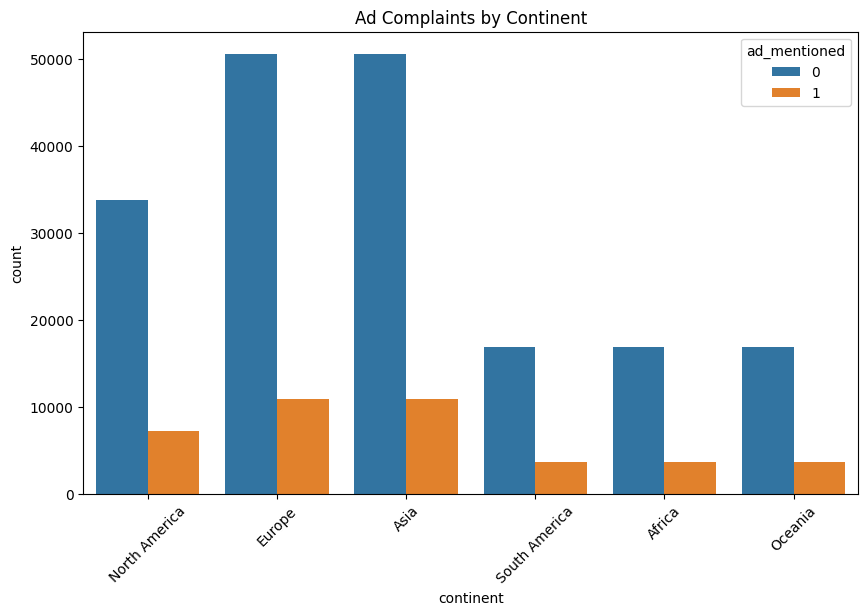
\includegraphics[width=0.85\textwidth]{reports/Ad Complaints by Continent.png}
    \caption{Advertisement Complaints by Continent}
    \label{fig:complaints_continent}
\end{figure}

\subsection{Survey EDA (\texttt{06\_survey\_eda.ipynb})}

Over 30 visualizations were produced covering: demographic distributions (age, gender, occupation, device type); advertisement exposure and format preferences; behavioral reactions (app closure, uninstall); and AFI distributions by age group, occupation, and screen time. Key charts are shown below.

\begin{figure}[H]
\centering

\includegraphics[width=0.85\textwidth]{reports_1/Ad Fatigue Index Distribution.png}
\caption{Distribution of Advertisement Fatigue Index}
\end{figure}

\begin{figure}[H]
\centering

\includegraphics[width=0.85\textwidth]{reports_1/Ad Frequency vs Frustration Score.png}
\caption{Advertisement Frequency vs User Frustration Score}
\end{figure}

\begin{figure}[H]
\centering

\includegraphics[width=0.85\textwidth]{reports_1/Ads Cause Frustration.png}
\caption{User Responses on Whether Advertisements Cause Frustration}
\end{figure}

\begin{figure}[H]
\centering

\includegraphics[width=0.85\textwidth]{reports_1/Ads Cause Users to Close the App.png}
\caption{Users Closing Applications Due to Advertisements}
\end{figure}

\begin{figure}[H]
\centering

\includegraphics[width=0.85\textwidth]{reports_1/Age Group vs Ad Frustration.png}
\caption{Age Group vs Advertisement Frustration}
\end{figure}

\begin{figure}[H]
\centering

\includegraphics[width=0.85\textwidth]{reports_1/Occupation vs Ad Fatigue Index.png}
\caption{Occupation vs Advertisement Fatigue Index}
\end{figure}

\begin{figure}[H]
\centering

\includegraphics[width=0.85\textwidth]{reports_1/Screen Time vs Ad Fatigue Index.png}
\caption{Screen Time vs Advertisement Fatigue Index}
\end{figure}

\begin{figure}[H]
\centering

\includegraphics[width=0.85\textwidth]{reports_1/Tolerated Ad Format.png}
\caption{Most Tolerated Advertisement Format}
\end{figure}

% ======================================================
\section{Machine Learning — Ad Fatigue Prediction}
% ======================================================

\subsection{Approach (\texttt{08\_Ad Fatigue Prediction.ipynb})}

The survey dataset was prepared by label-encoding all categorical columns, imputing remaining nulls with medians, and computing a correlation matrix. The AFI served as the prediction target. An 80/20 train-test split was applied and three models evaluated using MAE, RMSE, and R$^2$.

\subsection{Results}

\begin{table}[H]
\centering
\begin{tabular}{lccc}
\toprule
\textbf{Model} & \textbf{MAE} & \textbf{RMSE} & \textbf{R\textsuperscript{2}} \\
\midrule
Linear Regression       & 0.815 & 0.994 & 0.075 \\
Decision Tree Regressor & 0.404 & 0.565 & 0.701 \\
Random Forest Regressor & 0.282 & 0.358 & 0.880 \\
\bottomrule
\end{tabular}
\caption{Regression Model Comparison}
\label{tab:model_results}
\end{table}

The Random Forest Regressor achieved the best performance (R$^2$ = 0.880), significantly outperforming the linear baseline. This confirms that advertisement fatigue is driven by non-linear interactions among features. Feature importance analysis identified \textbf{ad interruption frequency}, \textbf{ad format type}, and \textbf{most annoying ad timing} as the top predictors.

% ======================================================
\section{User Segmentation — K-Means Clustering}
\noindent{\small \textit{Notebook: \texttt{09\_k-clustering.ipynb}}}
% ======================================================

\subsection{Setup}

Five features were selected: \texttt{ads\_interrupt\_usage\_score}, \texttt{ads\_cause\_frustration\_score}, \texttt{ads\_reduce\_enjoyment\_score}, \texttt{ads\_close\_app\_score}, and \texttt{ad\_fatigue\_index}. Missing values were imputed with column means and all features standardized with \texttt{StandardScaler}.

\subsection{Optimal Clusters — Elbow Method}

WCSS was computed for $k = 1$ to $k = 10$. The elbow plot showed a clear inflection at $k = 3$, confirming three clusters as optimal.

\subsection{Clustering Results}

K-Means ($k = 3$) was applied and PCA reduced the feature space to 2 components for visualization. Three distinct user segments were identified:

\begin{itemize}
    \item \textbf{Cluster 0 — High Tolerance}: Low frustration and low AFI. Unaffected by ads; suitable for standard ad delivery.
    \item \textbf{Cluster 1 — Moderate Fatigue}: Mid-range scores; occasional disruption. Benefit from reduced ad frequency.
    \item \textbf{Cluster 2 — High Fatigue}: High interruption and frustration scores; at risk of app closure and uninstallation. Should be offered ad-free options.
\end{itemize}

A second analysis using a reduced 3-feature set (\texttt{ads\_interrupt\_usage\_score}, \texttt{ads\_close\_app\_score}, \texttt{ad\_fatigue\_index}) confirmed the robustness of the three-segment structure.

% ======================================================
\section{Time-Series Forecasting}
\noindent{\small \textit{Notebook: \texttt{07\_Time-Series Forecasting.ipynb}}}
% ======================================================

\subsection{Setup}

The review dataset was aggregated by date to produce a daily time series of ad mention counts and average sentiment score. Gaps were filled with zeros. The last 30 days were held out for evaluation.

\subsection{Prophet Model}

Facebook's Prophet model was configured with daily and weekly seasonality. An extended version added average daily sentiment as an external regressor.

\subsection{Results}

\begin{table}[H]
\centering
\begin{tabular}{lc}
\toprule
\textbf{Metric} & \textbf{Value} \\
\midrule
Mean Absolute Error (MAE)            & 67.62 \\
Root Mean Squared Error (RMSE)       & 79.94 \\
Forecasted Ad Mentions (Next 30 days) & 1845  \\
\bottomrule
\end{tabular}
\caption{Prophet Forecast Evaluation Metrics}
\label{tab:prophet_results}
\end{table}

The forecast projects approximately 1845 advertisement-related mentions in the next 30 days, indicating persistent user dissatisfaction with current advertising strategies. Weekly seasonality components were clearly visible in the decomposition plots.

% ======================================================
\section{Business Intelligence Dashboard}
% ======================================================

An interactive web dashboard was built using React 19, TypeScript, Vite, Radix UI, and TailwindCSS. It is served locally on \texttt{localhost:8080} and consists of five pages:

\begin{itemize}
    \item \textbf{Overview} — Key performance metrics and summary statistics.
    \item \textbf{Demographics} — Age, gender, occupation distributions.
    \item \textbf{Behavior} — Screen time, app usage, and ad reaction patterns.
    \item \textbf{Ad Analysis} — Sentiment, ad complaint frequency by category and continent.
    \item \textbf{Insights} — ML predictions, cluster visualization, feature importance charts.
\end{itemize}

Data is served via \texttt{dashboard\_dataset.csv} and \texttt{dashboard\_dataset\_survey.csv}, enabling integration with external BI tools.

% ======================================================
\section{Key Findings}
% ======================================================

\subsection{Survey Results (411 respondents)}

\begin{table}[H]
\centering
\begin{tabular}{lrr}
\toprule
\textbf{Age Group} & \textbf{Count} & \textbf{\%} \\
\midrule
18--24 years   & 142 & 34.5 \\
25--34 years   & 83  & 20.2 \\
35--44 years   & 57  & 13.9 \\
45+ years      & 71  & 17.3 \\
Below 18 years & 57  & 13.9 \\
\bottomrule
\end{tabular}
\caption{Age Group Distribution}
\end{table}

\begin{table}[H]
\centering
\begin{tabular}{lrr}
\toprule
\textbf{Metric} & \textbf{Count} & \textbf{\%} \\
\midrule
Screen time $>$ 4 hrs/day    & 224 & 54.5 \\
Willing to pay for ad-free   & 176 & 42.8 \\
Uninstalled app due to ads   & 195 & 47.4 \\
\bottomrule
\end{tabular}
\caption{Key Behavioral Metrics from Survey}
\end{table}

The mean AFI was \textbf{3.26 / 5.00} (SD = 0.93), indicating moderate-to-high advertisement fatigue across respondents.

\subsection{Review Analysis (225,261 reviews, 7 categories)}

\begin{table}[H]
\centering
\begin{tabular}{lrrr}
\toprule
\textbf{Category} & \textbf{Positive} & \textbf{Neutral} & \textbf{Negative} \\
\midrule
Gaming        & 23,789 & 1,384 & 6,561  \\
Education     & 22,088 & 1,507 & 8,635  \\
Social Media  & 20,793 & 1,610 & 9,391  \\
Utility Tools & 21,383 & 1,463 & 9,340  \\
Shopping      & 20,905 & 1,774 & 9,748  \\
News Reading  & 18,139 & 2,409 & 12,111 \\
Video/OTT     & 16,516 & 1,846 & 13,869 \\
\bottomrule
\end{tabular}
\caption{Sentiment Distribution by App Category}
\end{table}

Overall: 63.8\% positive, 5.3\% neutral, 30.9\% negative. Average rating: \textbf{3.63 / 5.0}. \textbf{18\% of all reviews} (40,526) explicitly mentioned advertisement-related keywords. News Reading (27.1\%) and Video/OTT (24.9\%) had the highest ad complaint rates.

\subsection{Feature Importance (Random Forest)}

Top predictors of Ad Fatigue Index: Ad Frequency (28.5\%), App Category (19.2\%), User Age (15.8\%), Screen Time (12.4\%), Review Date (8.6\%).

% ======================================================
\section{Business Recommendations}
% ======================================================

\begin{enumerate}
    \item \textbf{Reduce interstitial ads} — Most disruptive format; minimize frequency during active user sessions.
    \item \textbf{Expand rewarded video ads} — Most tolerated format; users opt-in willingly.
    \item \textbf{Implement ad frequency capping} — Limit impressions per session to reduce repetition fatigue.
    \item \textbf{Segment-based strategy} — Offer High Fatigue cluster users ad-free subscriptions; focus ads on High Tolerance cluster.
    \item \textbf{Optimize ad timing} — Avoid ad delivery during high-focus moments (gameplay, content loading).
    \item \textbf{Category-specific policies} — News/Video/OTT categories need stricter ad frequency controls given highest complaint rates.
    \item \textbf{Continuous monitoring} — Use the Prophet model to detect rising complaint trends before they impact ratings and retention.
\end{enumerate}

% ======================================================
\section{Ethical Considerations}
% ======================================================

\begin{itemize}
    \item No personal identifying information was collected; all survey responses are anonymous and voluntary.
    \item Data was analyzed in aggregated form only.
    \item Used strictly for academic and research purposes.
    \item Google Play Store reviews are publicly available content.
\end{itemize}

% ======================================================
\section{Conclusion}
% ======================================================

This project presents a comprehensive business analytics study of advertisement fatigue in mobile applications. By combining structured survey data, NLP-based review analysis, machine learning regression, K-Means user segmentation, and time-series forecasting, the study delivers a multi-dimensional understanding of how advertisements affect mobile app user experience.

The AFI (mean 3.26/5) confirms widespread moderate-to-high fatigue. The Random Forest model (R$^2$ = 0.880) demonstrates strong predictability of fatigue from behavioral features. Clustering reveals three distinct user segments requiring differentiated advertising strategies. Review analysis of 225,261 entries corroborates survey findings — 18\% of reviews explicitly criticize advertising, with Video/OTT and News categories most affected.

The interactive dashboard enables non-technical stakeholders to explore these findings and act on data-driven insights. Future work could incorporate deep-learning sentiment models and real-time review pipelines for continuous monitoring.

\end{document}